\chapter{Resultats}

\section{Cas de la Terra a Mart}
\begin{itemize}
	\item Sortida: $t_{1}=$2020 Juliol 19
	\item Arribada: $t_{2}=$2021 Gener 25
\end{itemize}
\begin{table}[h!]
	\centering
	\begin{tabular}{ |c|c|c|c|c|c|}
		\hline
		$a$ & $e$ & $\theta_{1}$ & $\omega$ & $i$ & $\Omega$ \\ \hline
		$1.33073$ AU  & $0.23629$ & $359.613^{\circ}$ & $0.387^{\circ}$ & $1.434^{\circ}$ & $296.515^{\circ}$ \\ \hline
	\end{tabular}
	\caption{Elements orbitals del primer cas resolt}
\end{table}

\section{Cas de Mart a Júpiter}
\begin{itemize}
	\item Sortida: $t_{1}=$2026 Juny 05
	\item Arribada: $t_{2}=$2029 Abril 25
\end{itemize}
\begin{table}[h!]
	\centering
	\begin{tabular}{ |c|c|c|c|c|c|}
		\hline
		$a$ & $e$ & $\theta_{1}$ & $\omega$ & $i$ & $\Omega$ \\ \hline
		$3.45405$ AU  & $0.59043$ & $356.872^{\circ}$ & $176.203^{\circ}$ & $7.508^{\circ}$ & $207.127^{\circ}$ \\ \hline
	\end{tabular}
	\caption{Elements orbitals del segon cas resolt}
\end{table}

\section{Cas 1 de Mart a Júpiter}
\begin{itemize}
	\item Sortida: $t_{1}=$2037 Octubre 25
	\item Arribada: $t_{2}=$2039 Octubre 15
\end{itemize}
\begin{table}[h!]
	\centering
	\begin{tabular}{ |c|c|c|c|c|c|}
		\hline
		$a$ & $e$ & $\theta_{1}$ & $\omega$ & $i$ & $\Omega$ \\ \hline
		$3.87684$ AU  & $0.64755$ & $392.516^{\circ}$ & $317.644^{\circ}$ & $1.267^{\circ}$ & $52.502^{\circ}$ \\ \hline
	\end{tabular}
	\caption{Elements orbitals del cas 1}
\end{table}

\section{Cas 2 de la Terra a Mart}
\begin{itemize}
	\item Sortida: $t_{1}=$2033 Març 13
	\item Arribada: $t_{2}=$2033 Agost 05
\end{itemize}
\begin{table}[h!]
	\centering
	\begin{tabular}{ |c|c|c|c|c|c|}
		\hline
		$a$ & $e$ & $\theta_{1}$ & $\omega$ & $i$ & $\Omega$ \\ \hline
		$1.34585$ AU  & $0.26502$ & $347.845^{\circ}$ & $12.155^{\circ}$ & $2.154^{\circ}$ & $172.263^{\circ}$ \\ \hline
	\end{tabular}
	\caption{Elements orbitals del cas 2}
\end{table}

\section{Cas 3 de la Terra a Mart}
\begin{itemize}
	\item Sortida: $t_{1}=$2031 Gener 23
	\item Arribada: $t_{2}=$2031 Agost 01
\end{itemize}
\begin{table}[h!]
	\centering
	\begin{tabular}{ |c|c|c|c|c|c|}
		\hline
		$a$ & $e$ & $\theta_{1}$ & $\omega$ & $i$ & $\Omega$ \\ \hline
		$1.24568$ AU  & $0.20996$ & $1.674^{\circ}$ & $358.471^{\circ}$ & $2.293^{\circ}$ & $122.188^{\circ}$ \\ \hline
	\end{tabular}
	\caption{Elements orbitals del cas 3}
\end{table}

\section{Cas 4 de la Terra a Mart}
\begin{itemize}
	\item Sortida: $t_{1}=$2025 Juliol 18
	\item Arribada: $t_{2}=$2025 Octubre 21
\end{itemize}
\begin{table}[h!]
	\centering
	\begin{tabular}{ |c|c|c|c|c|c|}
		\hline
		$a$ & $e$ & $\theta_{1}$ & $\omega$ & $i$ & $\Omega$ \\ \hline
		$1.07039$ AU  & $0.46551$ & $112.076^{\circ}$ & $67.350^{\circ}$ & $0.563^{\circ}$ & $115.868^{\circ}$ \\ \hline
	\end{tabular}
	\caption{Elements orbitals del cas 4}
\end{table}

\section{Cas 5 de la Terra a Venus}
\begin{itemize}
	\item Sortida: $t_{1}=$2023 Maig 27
	\item Arribada: $t_{2}=$2023 Novembre 01
\end{itemize}
\begin{table}[h!]
	\centering
	\begin{tabular}{ |c|c|c|c|c|c|}
		\hline
		$a$ & $e$ & $\theta_{1}$ & $\omega$ & $i$ & $\Omega$ \\ \hline
		$0.86221$ AU  & $0.23212$ & $147.050^{\circ}$ & $32.951^{\circ}$ & $1.678^{\circ}$ & $65.165^{\circ}$ \\ \hline
	\end{tabular}
	\caption{Elements orbitals del cas 5}
\end{table}

\section{Cas 6 de Mart a la Terra}
\begin{itemize}
	\item Sortida: $t_{1}=$2033 Gener 18
	\item Arribada: $t_{2}=$2033 Agost 28
\end{itemize}
\begin{table}[h!]
	\centering
	\begin{tabular}{ |c|c|c|c|c|c|}
		\hline
		$a$ & $e$ & $\theta_{1}$ & $\omega$ & $i$ & $\Omega$ \\ \hline
		$1.31415$ AU  & $0.24918$ & $191.345^{\circ}$ & $207.993^{\circ}$ & $1.696^{\circ}$ & $154.559^{\circ}$ \\ \hline
	\end{tabular}
	\caption{Elements orbitals del cas 6}
\end{table}

\section{Cas 7 de Mart a la Terra}
\begin{itemize}
	\item Sortida: $t_{1}=$2030 Novembre 20
	\item Arribada: $t_{2}=$2031 Juliol 06
\end{itemize}
\begin{table}[h!]
	\centering
	\begin{tabular}{ |c|c|c|c|c|c|}
		\hline
		$a$ & $e$ & $\theta_{1}$ & $\omega$ & $i$ & $\Omega$ \\ \hline
		$1.31613$ AU  & $0.26617$ & $184.700^{\circ}$ & $220.499^{\circ}$ & $2.572^{\circ}$ & $103.210^{\circ}$ \\ \hline
	\end{tabular}
	\caption{Elements orbitals del cas 7}
\end{table}
\begin{figure}[H]
	\centering
	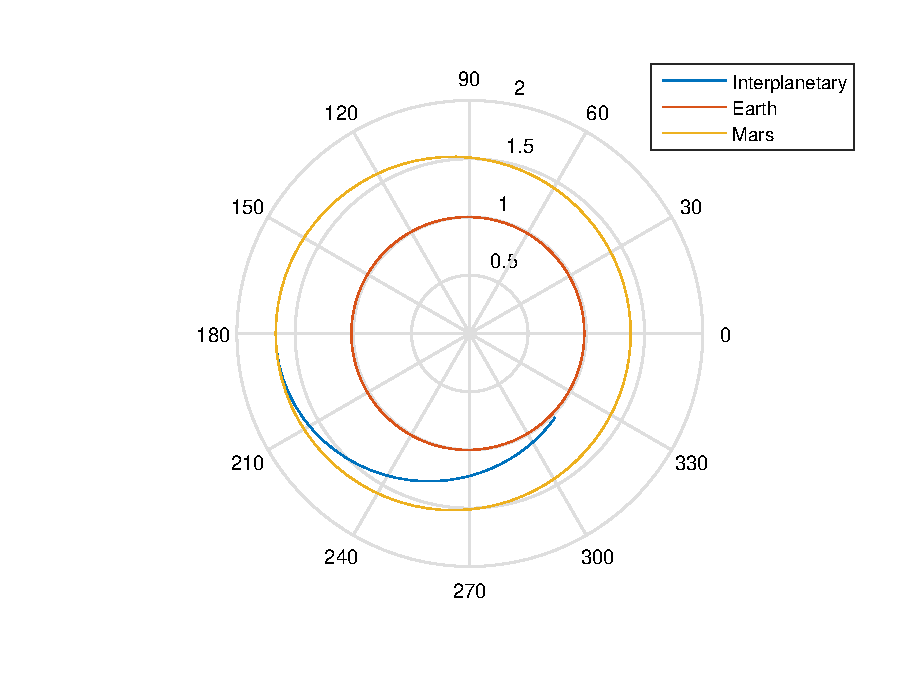
\includegraphics[scale=0.95]{./plots/cas7}
	\caption{Òrbita interplanetària del cas 7}
\end{figure}